\section{Introduction}

Over the last decade global interest in wave energy has grown
considerably, with the Ocean Energy Systems executive committee
setting a goal of 300GW of installed ocean energy capacity by 2050
\citep[]{huckerbyInternationalVisionOcean2017}. This has been driven
by concerns about greenhouse-gas driven climate change, carbon-based
energy price volatility, and a growing emphasis on the value of
diversifying energy sources. Wave energy is seen as particularly
valuable for its predictability and reliability on timescales of hours
to a few days \citep{parkinsonIntegratingOceanWave2015}, and for the
fact that the resource is concentrated along coastlines where large
fractions of the world's populations live. Furthermore, the
U.S. Department of Energy has recently initiated a ``Powering the Blue
Economy'' initiative designed to support the development of
technologies that provide power to unique market applications such as
desalination, ocean sensing, aquaculture, and coastal community
resiliency \citep{PBE_REPORT}. Wave energy technology is still at an
early-stage of technology development with a wide-range of device
archetypes under active development
\citep[]{babaritOceanWaveEnergy2017}.

The 2011 DOE-funded U.S. wave resource assessment provided the first
comprehensive estimate of the nation’s wave energy resource, and has
been an important reference for motivating private and public
investment in wave energy research ever since
\citep[]{EPRIwaveresource2011}. In 2013 the National Academy of
Sciences published a review of the DOE’s marine energy resource
assessments including: tidal, ocean current, in-stream river, ocean
thermal energy, and the 2011 wave energy resource assessment
\citep{nationalresearchcouncilEvaluationDepartmentEnergy2013}.  The
National Academy generally found that the resource assessments provide
“a useful contribution to understanding the distribution and possible
magnitude of marine and hydrokinetic energy sources in the United
States,” but also had specific technical critiques of each assessment,
and of the comparability of the results between each of the
assessments.

In the case of wave energy, the National Academy’s review points out that
because the method used did not account for wave direction, it “has the
potential to double-count a portion of the wave energy”. At the same
time, in discussions with several wave energy experts, we found
complimentary criticisms such as: the idea that the
integration-contour where wave energy is calculated is arbitrary, and
furthermore that most methodologies for performing this integration do
not account for the ``recovery'' of the wave-field due to local winds
down-wave from that contour. The primary objective of this work is to
develop a methodology that resolves these questions and critiques so
that decision-makers and the international wave energy community has a
robust and consistent methodology for regional wave resource
assessment.

\subsection{International standards for wave resource assessment}

\note{Gabriel: I just wanted to make note of a few things that I think need to be included in this. I think we need to define 'theoretical resource' using the IEC definition. Maybe we don't also need 'technical' and 'practical resource'? But their definitions do help clarify what is meant by 'theoretical'. I also think we need to include some reference to IEC-101 Table 1, and how our work compliments that document in general. This is one of the main places I get hung up: "why didn't IEC do this... because they were focused on project-scale".
}

The International Electrotechnical Commission's Technical Committee on
Marine Energy (TC114) has published the first edition of a wave
resource assessment technical specification that ``provides a uniform
methodology that will ensure consistency and accuracy in the
estimation, measurement, and analysis of the wave energy resource at
sites that could be suitable for the installation of Wave Energy
Converters (WECs), together with defining a standardised methodology
with which this resource can be described.'' The certified assessments
that are based on this document are expected to improve investor and
financier confidence, and thereby reduce the cost of marine
energy. Several works follow the IEC standards in characterizing the
wave resource at sites around the world
\citep{zhengAssessingChinaSea2013,neillWavePowerVariability2013,iglesiasWaveEnergyPotential2009,sierraWaveEnergyResource2013,robertsonCharacterizingShoreWave2014,internationalelectrotechnicalcommissionPart101Wave2015,yangCharacteristicsVariabilityNearshore2020,lokuliyana_sri_2020}.

However, because the current (first edition) of the
technical specification is focused on this objective, which is
relevant primarily at the project-scale, it does not currently
provides guidance on estimating total aggregated available power at the regional
scale.
%except to say that ``the effects of the WEC array on wave propagation should be included in the numerical model''. This is not directly related to the aggregation of the resource, I think we need to remove this. 

TC114's wave resource assessment technical specification does define
three classes of resource assessment: reconnaissance, feasibility, and
design. These are meant to be applied at successively smaller scales
for the purpose of: identifying regions that are promising, then
identifying a specific site of interest, then designing the project
layout. However, because the reconnaissance resource
assessment as defined there does not provide guidance on estimating
the total energy at large scales (i.e., it does not specify a method
for performing a line-integral), it is distinct from what we define
here as ``regional'' resource assessment. In particular, we identify
two important types of resource assessment that are motivated by
distinct goals:

\begin{enumerate}
\item Global, regional, and national assessments (hereafter, collectively ‘regional’ assessments) that quantify the total theoretical resource for a relatively long section of coastline (i.e., $>$O(100 km)). Most importantly, regional assessments provide an estimate of the total power available in the wave field for the region of interest.
\item Site resource assessments provide a collection of resource details that are useful for estimating the site’s power production potential and for project design. Most importantly, site assessments provide a joint probability distribution of wave energy period and wave height that can be used with a device ‘power matrix’ to calculate the project’s annual energy production.
\end{enumerate}

These assessments are valuable for different purposes. Regional assessments are the foundation of more detailed market research (such as site assessments), they motivate regional planning, and provide justification for government investment \citep[e.g., ][]{EPRIwaveresource2011,gunnQuantifyingGlobalWave2012,regueroGlobalWavePower2015,motaWaveEnergyPotential2014}. Site assessments provide data needed for feasibility and design studies that are critical to obtaining project financing and investment \citep[]{robertsonCharacterizingShoreWave2014,iglesiasWaveEnergyPotential2009}.

\noindent\rule{12cm}{0.4pt}

A detail that confounds unifying these two approaches is the fact that wave energy flux is a directional quantity. This means that - in order to avoid double counting - regional totals must account for the directionality by performing a line-integral. On the other hand, for site assessments involving sparsely positioned omni-directional devices (i.e., devices that absorb energy equally in all directions), wave directionality does not have a significant impact on the project’s technical potential. With this understanding and motivated by a desire to address the needs of the industry where it is now (i.e., most projects involve 10 or less devices), the first edition of the International Electrotechnical Commission’s resource assessment technical specification does not explicitly account for directionality or array effects \citep[]{internationalelectrotechnicalcommissionPart101Wave2015}. While the IEC site assessment methodology has these limitations, it has been developed through a consensus process that encourages widespread adoption and consistency. The methodology for regional assessments, on the other hand, has not been developed by consensus, which has led to inconsistent approaches and confusion when comparing results.

\textcolor{green}{I have two comments on the above paragraph that I tried to address below.
\begin{itemize}
    \item IEC accounts for directionality in quantities such as $\theta_{Jmax}$, $d$, and mandating wave power roses. It does not have provisions for aggregating the resource spatially. I'll try to rephrase the above paragraph to reflect that.
    \item I do not think that ignoring integrated assessments is a limitation of IEC Technical Specifications, it is just a different focus area. 
\end{itemize}}

A detail that confound unifying these two approaches is the fact that wave energy flux is a directional and spatially varying quantity. This means that - in order to avoid double counting when computing the total resource - regional totals must account for the directionality by performing a line-integral. On the other hand, for site assessments involving sparsely positioned omni-directional devices (i.e., devices that absorb energy equally in all directions), wave directionality does not have a significant impact on the project’s technical potential. With this understanding and motivated by a desire to address the needs of the industry where it is now (i.e., most projects involve 10 or less devices), the first edition of the International Electrotechnical Commission’s resource assessment technical specification does not explicitly provide guidance on regional resource estimates or explicitly account for array effects \citep[]{internationalelectrotechnicalcommissionPart101Wave2015}. In other words, an assessment following IEC will report wave energy density but not wave energy potential. The IEC site assessment methodology has been developed through a consensus process that encourages widespread adoption and consistency. The methodology for regional assessments, on the other hand, has not been developed by consensus, which has led to inconsistent approaches and confusion when comparing results.

\noindent\rule{12cm}{0.4pt}

We undertake the task of establishing a consistent regional wave
resource assessment methodology by first pointing out that the wave
resource for a region of water is composed of two parts (Figure
\ref{fig:diagram:west-eez}): 1) the ‘remote resource’, which is the
wave energy created by winds outside the region — e.g., by storms in
the distant open-ocean — that propagates into the region
\citep{gunnQuantifyingGlobalWave2012,
hemerRevisedAssessmentAustralia2017}, and 2) the ‘local resource’,
which is the wave energy created by winds within the region
itself. The majority of existing wave resource assessments have
considered the remote resource only. While neglecting the local
resource may be reasonable for small projects, the fact that it has
been ignored (often implicitly) has raised many questions and led to
confusion about wave resource assessment methodology. The primary
objective of this work is to develop a methodology for quantifying
both the remote and local resource explicitly, and thereby resolve
lingering questions regarding the details of regional resource
assessment.

\begin{figure}[ht]
  \centering
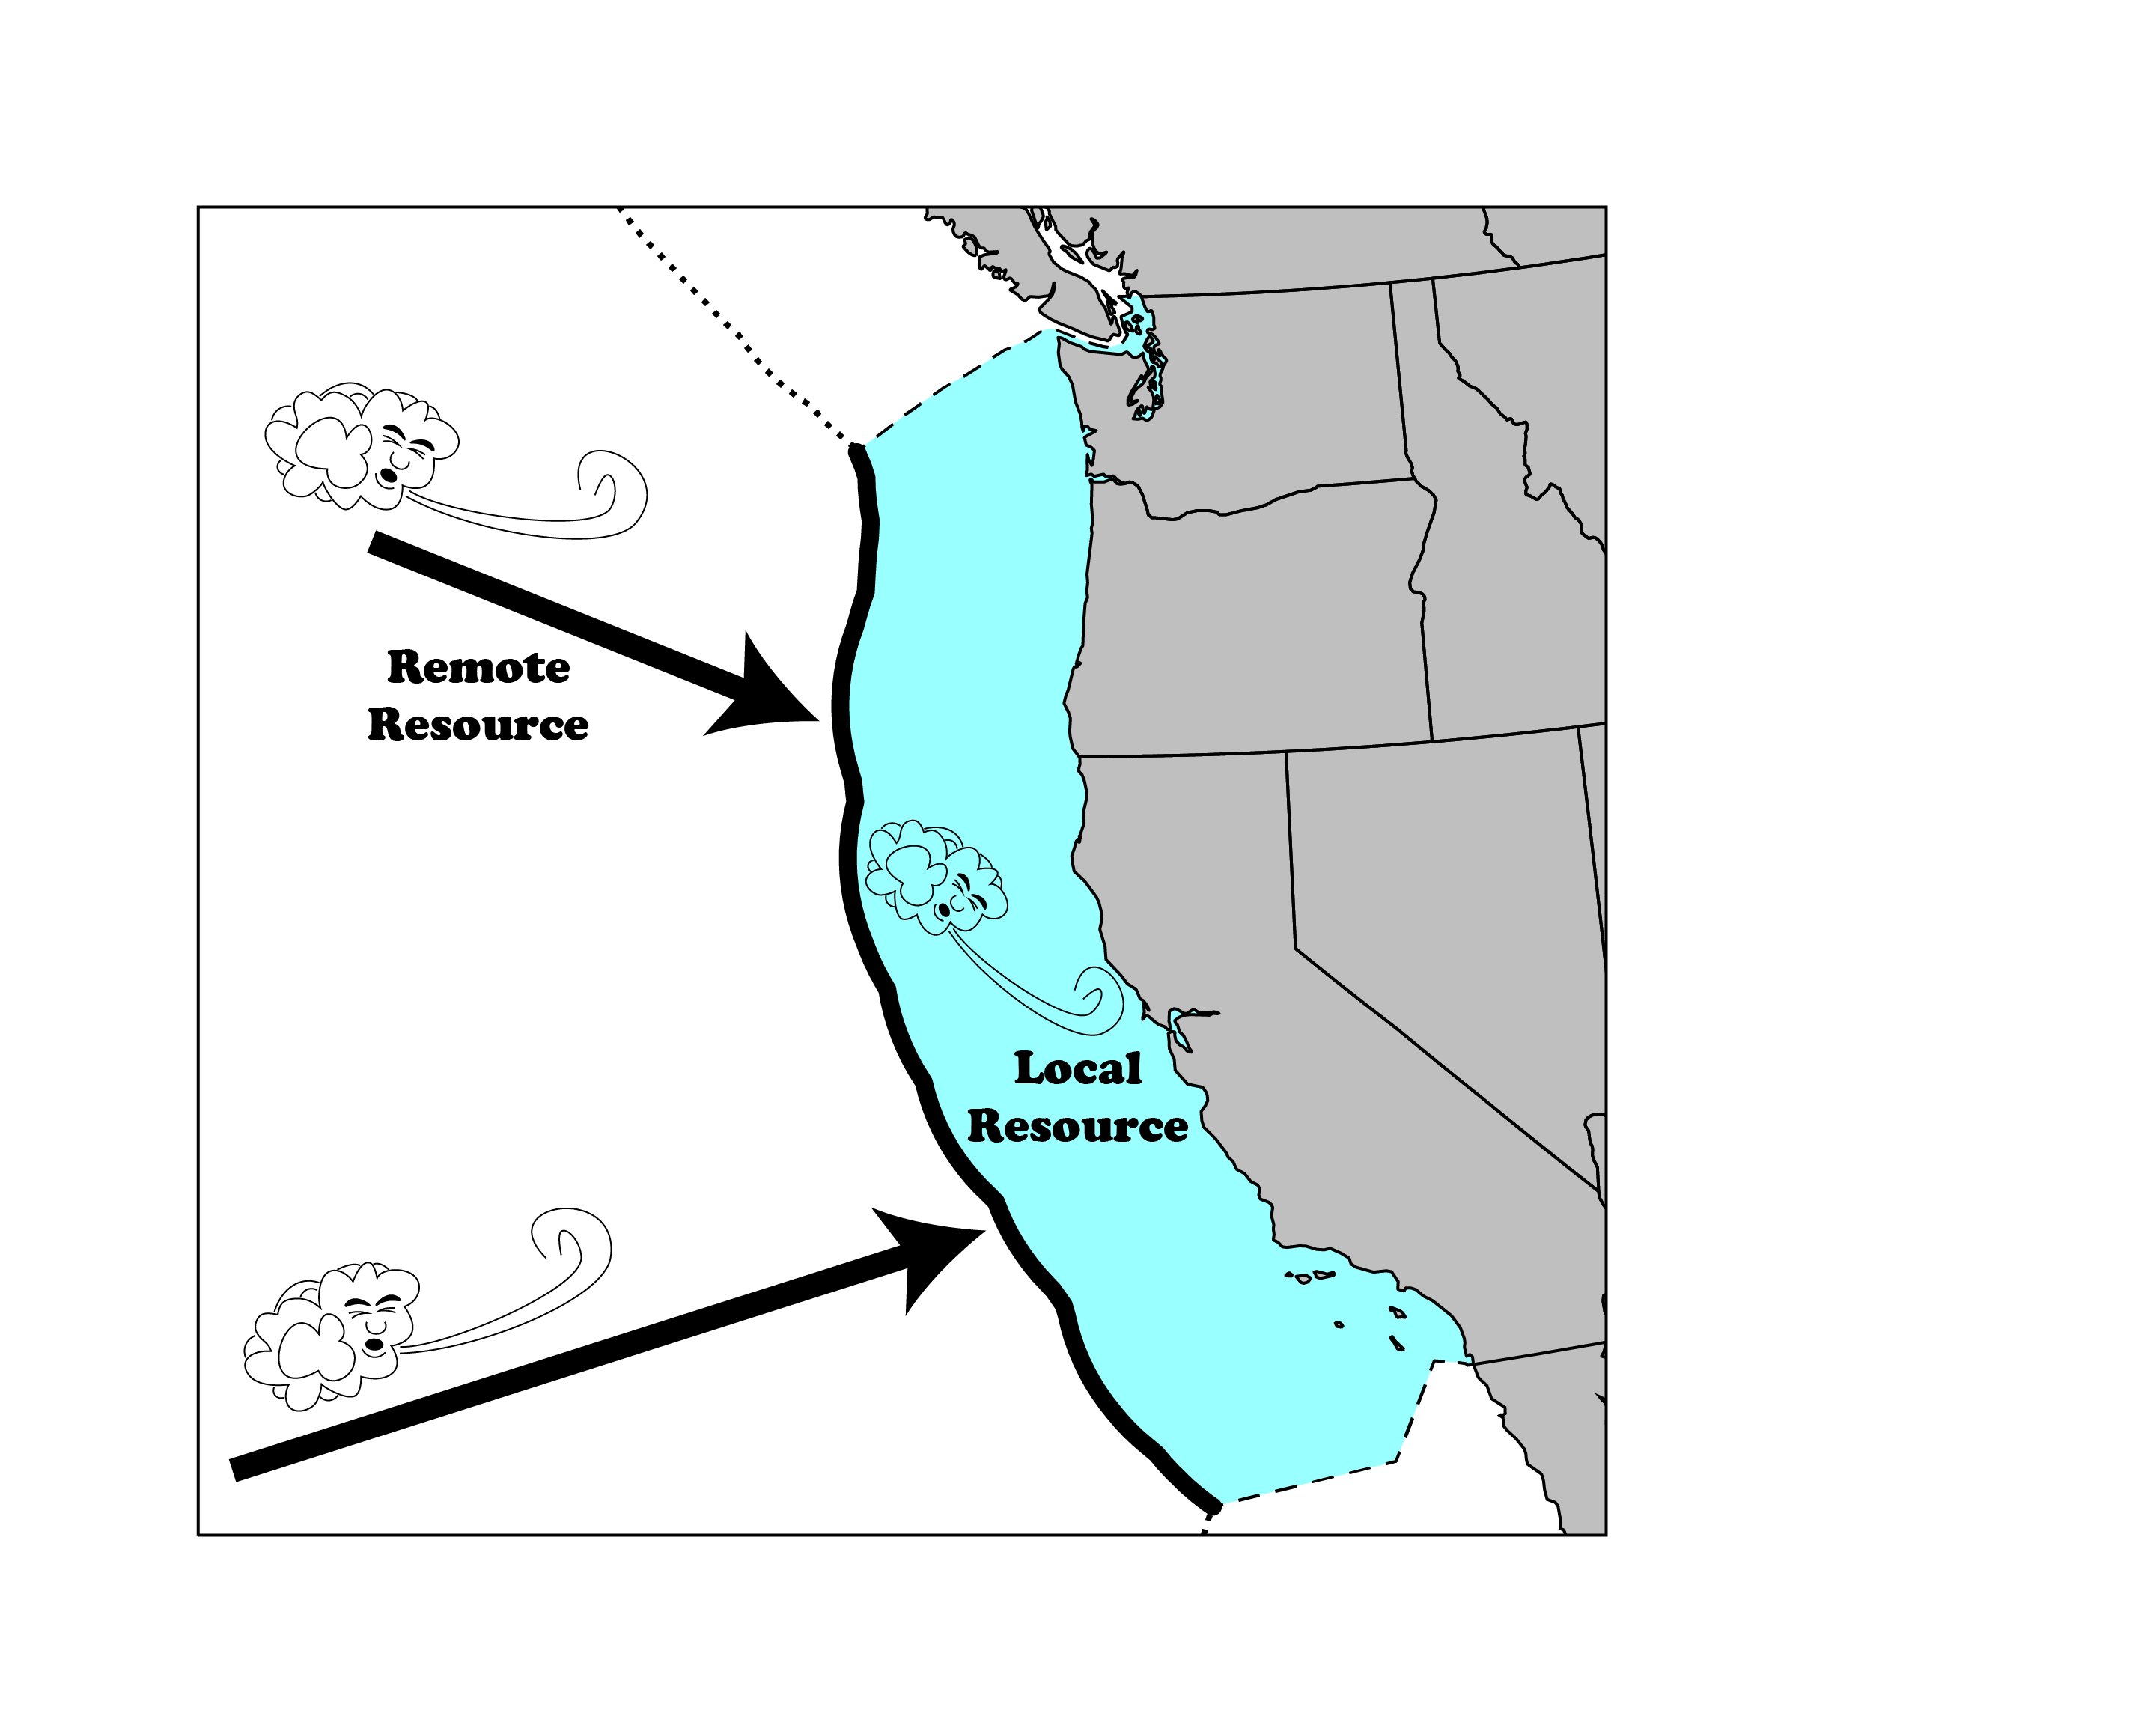
\includegraphics[width=0.9\linewidth]{../diagram/EEZ_contour03_edit01.png}
  \caption{A diagram depicting the U.S. West Coast’s ‘remote’ (arrows) and ‘local’ (cyan region) resource.}
  \label{fig:diagram:west-eez}
\end{figure}

A secondary objective of this work is to provide a refined estimate of
the U.S. wave resource based on this new method, and new model
results. A tertiary objective is to provide guidance that helps
address limitations in site assessment, which we hope will eventually
lead to a unified methodology for site and regional wave resource
assessment.

These objectives are accomplished by first discussing the details of regional assessments (section 2), and then presenting our proposed approach (section 3). In section 4, we present the results of this approach applied to each region of the U.S. coastline in comparison to alternate methods that have been used. Section 5 provides a detailed discussion of the results, including a justification for the proposed approach, and a summary of how the proposed approach can be applied in different scenarios. We conclude with a summary of results, the proposed methodology, and a view toward how to unify wave energy site and resource assessment

% Need to define `theoretical resource assessment'
\noindent\rule{12cm}{0.4pt}

\textcolor{green}{No need to say this again. I like you you explained the three points above. Consider removing this.}
This paper has two primary objectives: 1) to define a new methodology for quantifying theoretical wave resource that addresses critiques of previous approaches that can be applied at any scale, and 2) to apply that method to all U.S. regions to obtain an updated assessment of the nation's wave energy potential (theoretical resource).

\noindent\rule{12cm}{0.4pt}


\subsection{IEC Stuff?}
\textcolor{green}{I would remove this section. I think the differences between the IEC and this paper are clearly stated above. Some but not all text can make it to the previous section. I outlined in green what I think should be kept.}

During these early years of wave energy research and development, it has been
important to quantify the wave energy resource so that decision makers can begin
to understand the market opportunity of this new technology and so that project developers can identify development sites. In this context the international electrotechnical commissions's technical committee on marine energy (IEC TC114) has been working to clarify the terminology for describing marine energy, and to define the methods for quantifying its potential.

This task is complicated by a need to quantify the opportunity at multiple scales (from the scale of a single project or device, all the way up to regional and national assessments), and a need to consider technical and practical constraints on the opportunity. To clarify this space, IEC TC114 has defined three types of resource assessment
\citep{internationalelectrotechnicalcommissionPartTerminology2011} \note{These
definitions are the ED2 defs, but this citation is the original. Need to update
once Ed-2 is published. Also: how do these definitions compare to what is used
for RA of wind/solar? Is that important?}:

\begin{itemize}
  \item the {\it theoretical resource} is the ``energy available in the resource''
  \item the {\it technical resource} is the ``proportion of the theoretical resource that can be captured using existing technology options without consideration of external constraints''
  \item the {\it practical resource} is the ``proportion of the technical resource that is available after consideration of external constraints''
  \end{itemize}

\textcolor{green}{
In the case of wave energy, the energy ``available'' is equivalent to the energy contained in the wave field because it is theoretically possible to extract all of the energy from the waves as originally demonstrated by the ``Salter Duck'' \citep{salterRecentProgressDucks1980}. This is in contrast to the ``Betz limit'' of wind energy, which states that a wind turbine cannot extract more than 59.3\% of the kinetic energy in the wind.} 

At the same time as defining these three types of RA, the IEC wave resource assessment TS also defines three {\em classes} of resource assessment, which are defined primarily in terms of uncertainty and numerical model resolution \citep{internationalelectrotechnicalcommissionPart101Wave2015}. However, because this document was written for the purposes of characterizing the resource in terms of statistics that are useful to wave energy project developers, it does not provide specific guidance on quantifying the total theoretical resource available on regional scales. 
IEC TC114 technical specifications were written primarily to serve the needs of  These classes are:
\begin{enumerate}
\item ``reconaissance'', high uncertainty, spatial-scale $>300 km$
\item ``feasibility'', medium uncertainty, spatial-scale $20- 500 km$
\item ``design'', low uncertainty, spatial-scale $<25 km$
\end{enumerate}

\textcolor{green}{Move this to the previous section:
All three of these classes deal directly with estimating wave resource parameters at specific sites, and the TS does not directly tackle the problem of quantifying the total wave resource at any of these scales.} Instead, each of the 

  \note{
    So, even though IEC says it is focused on theoretical RA, and even though it defines three 'classes' of RA, it doesn't really deal with the first two!
    }
  
technical resource is the portion of this which could be extracted with
technology that is available today, and the practical resource is the portion
of the technical resource that is available when considering the myriad of other social, political, logistical,
economic, and environmental constraints that exist. Due to the inherent challenges of
quantifying the technical and practical resource, most works have typically
focused on the theoretical resource.


\note{There is something here about the different goals of Regional resource assessment (basically this starts with a line-integral of the total theoretical resource), and that of project-scale RA (which typically uses a JPD -- and/or directional-spectrum, or other stats: Hs, Tp, mean-wave-direction, etc -- to characterize the resource). ... But this isn't how IEC-101 addresses it, and that doc doesn't provide clear guidance on the line-integral approach. The IEC table is defined primarily in terms of  `accuracy', but is the accuracy of these different `classes' of assessment really that different? What is meant by ``high/medium/low uncertainty''? Should we suggest revising the IEC TS to better reflect table \ref{tab:scale-type}? Rather than lumping it all into the current definitions? Should IEC even deal w/ regional-scale RA, or just focus on ``project-scale technical RA''? Is there value in IEC defining ``regional-scale technical RA''? ... Project-scale theoretical is easy from the method here.
  Also, 62600-101 says its focus is 'theoretical RA' but it does not provide clear guidance on how to do the line-integral, other than `you should account for array effects'. i.e.,  even though -101 says it is focused on 'theoretical resource', it doesn't actually help you {\em calculate} the total. How does this square with the definition of `theoretical resource' above?
}

% Could go into the debate between how to define technical vs. theoretical here?
% - in idealized scenarios existing tech can extract nearly 100% of energy
%   (i.e., for monochromatic waves), but much less
%   efficient for mixed-waves.
% - If we install enough rows of real devices, what is limit on energy we can
%   extract? <- does anyone know this?
%   Thus, defining technical resource is challenging, so an ad-hoc approach has
%   typically been used (e.g., "25% of theoretical"), and similar for practical
%   resource (e.g., "25% of technical") ... the Quadrennial Tech Review uses numbers like
%   these.

This work focuses on the theoretical resource assessment because this has been
the primary focus of previous resource assessments.
\note{Basically: we are starting with theoretical because there has been plenty of disagreement about how to do that right, and now we are trying to resolve those discrepancies before moving on to refining estimates of the others.}

\note{There is a lot of discussion about different types of RA: theoretical / technical / practical, stage 1,2,3, resource classification, difference between regional-scale and project-scale. How do we simplify all of this?! Do we address it directly, or skip it?}
% The right approach is probably to categorize 'regional-scale assessments'
% under 'stage 1, theoretical', and outside the scope of 'resource
% classification' (skip this).



\begin{table}[t]
  \begin{tabular}{l|c|cc|cc|cc|}
    \multicolumn{2}{c}{} & \multicolumn{6}{c}{Type} \\
    \cline{3-8}
    \multicolumn{2}{c|}{}  & \multicolumn{2}{c|}{Theoretical} & \multicolumn{2}{c|}{Technical}  & \multicolumn{2}{c|}{Practical}  \\
    \cline{2-8}
    \multirow{4}{*}[-1ex]{\rotatebox{90}{Scale}} & Global & &$\square$  &  & & &\\
    & Regional & &$\blacksquare$  &  & & & \\
    & \vdots & &$\square$  &  & & & \\
    & Project & TS & $\square$  & TS &  & TS &  \\
    \cline{2-8}
  \end{tabular}
  \centering
  \caption{The scale-vs-type conceptual space of resource-assessment. \note{Need to think more about how this fits with Table 1 in IEC wave RA (-101). That table is focused primarily on accuracy/uncertainty of the approach, but it also overlaps with scale (last column). We could either: a) include that table adjacent to this one, or somehow summarize it as a column or two here. But, mostly I think there is something here about how the ``accuracy-focused'' approach there is sorta outdated b/c we can now run fairly high-accuracy/resolution models at large-scale.} }
  \label{tab:scale-type}
\end{table}

%%% Local Variables:
%%% TeX-master: "wave_res"
%%% End:
